The extended analysis containing GW151226 lasted from December 3, 2015 - January 19, 2016 and
contained a total of 16.7 days of coincident detector data.
After category 1 vetoes were removed, 16 days of coincident data remained. After
category 2 vetoes were removed, 15.8 days of coincident remained and were used in the
final analysis.
This analysis time provided
an extended background estimation for the binary black hole merger GW151226 \cite{GW151226},
which was detected by the aLIGO interferometers on December 26, 2015.

The gating process used in the analysis containing GW151226 was different than that used in 
previous analyses. 
Instead of relying on an external process, such as Omicron, to identify large transients,
an internal test is used to find large excursions in the input data \cite{Usman:2015kfa}.
The time domain input
data are Fourier transformed into the frequency domain and whitened using the
measured power spectral density. The data are then inverse Fourier transformed back into
the time domain and compared to a threshold value set to perform comparably to the
Omicron gating process.
If the whitened data have excursions that exceed this threshold, a gating window is
constructed to remove these data from the input to the search.
Tests were done to ensure that loud signals would not be removed by the auto-gating process.

\section{BNS bin}

The BNS bin shows a slight improvement when data quality vetoes are included.
Figure \ref{fig:bns-bin-far-GW151226} shows the background distributions in the BNS
bin before and after removing data with vetoes. The most significant
effect is that the loudest event in the background is at a higher re-weighted SNR;
the loudest background event is at $\hat{\rho}_{c} =$ 10.96 rather
than $\hat{\rho}_{c} =$ 10.6.

\begin{figure}[!ht]%
\centering
  \subfloat[]{
  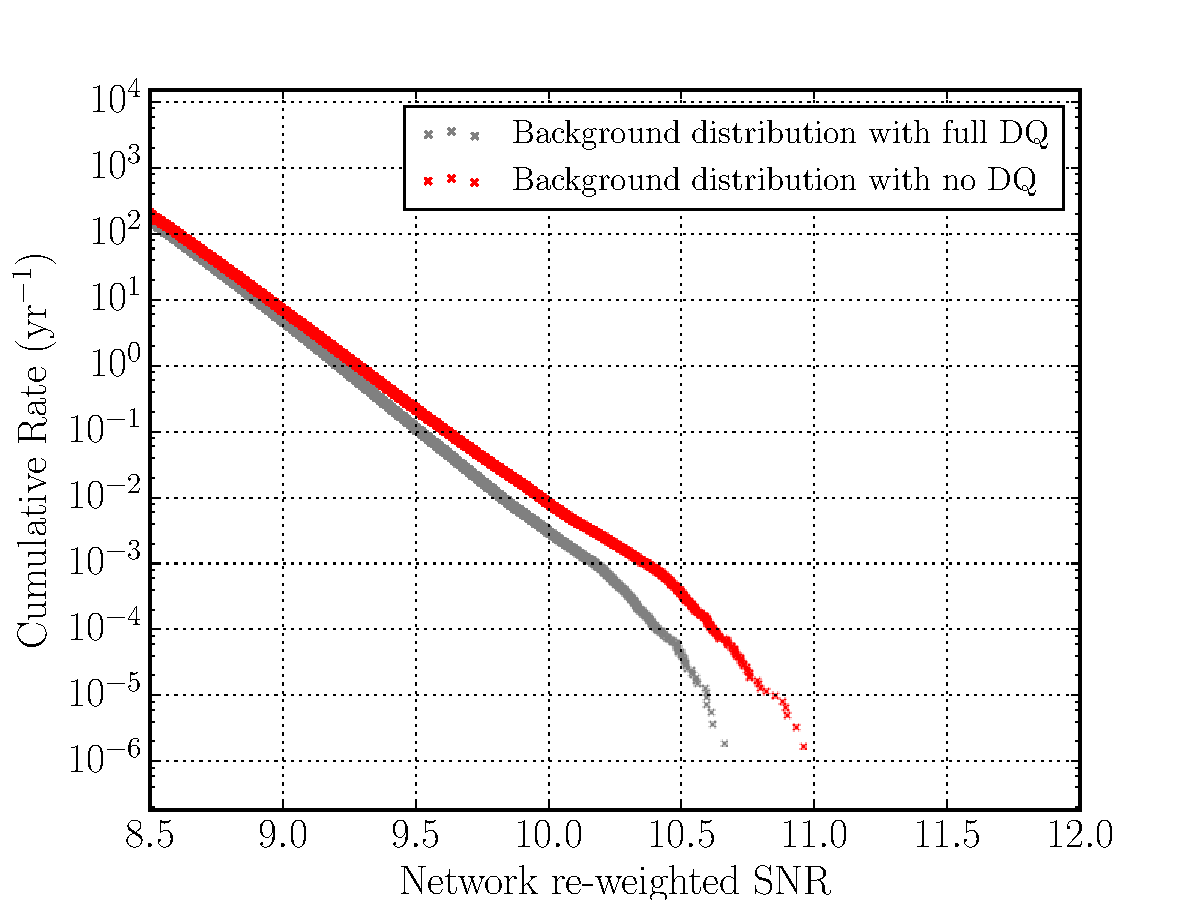
\includegraphics[width=0.495\textwidth]{figures/o1-cbc-dq-paper/bns_bin_GW151226_DQ_comparison}
  \label{subfig:bns-bin-gw151226-rate}
  }
  \subfloat[]{
  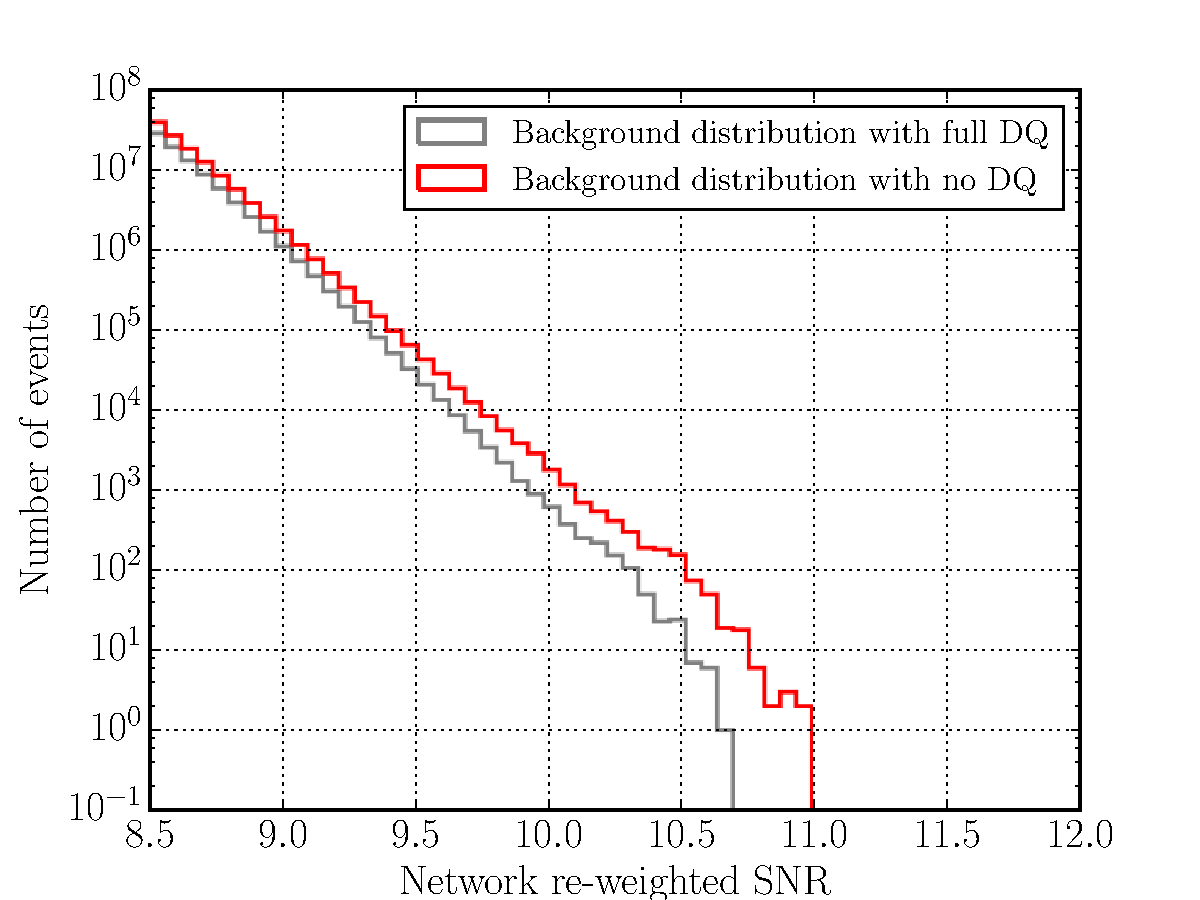
\includegraphics[width=0.495\textwidth]{figures/o1-cbc-dq-paper/bns_bin_GW151226_DQ_raw_hist}
  \label{subfig:bns-bin-gw151226-raw}
  }
  \caption[BNS bin histograms - GW151226 analysis]{The background distribution in the BNS bin before and after applying data quality (DQ) vetoes. %
           (\ref{subfig:bns-bin-gw151226-rate}) The cumulative rate of background triggers %
           in the BNS bin as a function of re-weighted SNR. %
           (\ref{subfig:bns-bin-gw151226-raw}) A histogram of background triggers %
           in the BNS bin. % 
           The red traces indicate the %
           distribution of background triggers without noisy data removed % 
           and the gray traces indicate the distribution %
           of background triggers with all data quality vetoes applied. %
           The BNS bin shows minimal improvement. %
           With noisy data removed, the loudest background event is at $\hat{\rho}_{c} =$ 10.6. %
           Without removing any data, the loudest background event is at $\hat{\rho}_{c} =$ 10.96. % 
          }
\label{fig:bns-bin-far-GW151226}
\end{figure}

Although the removal of problematic data has a visible impact on the background of the BNS bin,
the resulting distribution is still not limiting to the search. In both cases, the
hypothetical detection candidate at $\hat{\rho}_{c} =$ 11.3 would be the loudest event in the analysis.
The difference in false alarm rate is quantified in Table \ref{table:151226-bns-far}.

\begin{table}[!ht]%
  \begin{center}
    \begin{tabular}{lcc}
      \hline
      Analysis configuration & False alarm rate ($\mathrm{yr}^{-1}$) & False alarm probability \\ \hline
      All vetoes applied & $1.82\times10^{-6}$  & $7.60\times10^{-8}$ \\
      No CAT2 applied & $1.77\times10^{-6}$ & $7.48\times10^{-8}$ \\
      No CAT1 or CAT2 applied & $1.63\times10^{-6}$ & $7.18\times10^{-8}$ \\ \hline
    \end{tabular}
  \end{center}
  \caption[BNS bin FAR - GW151226 analysis]{Table of false alarm rates and probabilities at $\hat{\rho}_{c} =$ 11.3 for several analysis configurations. %
           The difference in false alarm rate between the different configurations is negligible %
           in the BNS bin.}
  \label{table:151226-bns-far}
\end{table}

\section{Bulk bin}

The bulk bin benefited from the application of data quality vetoes. Figure
\ref{fig:bulk-bin-far-GW151226} shows the bulk bin background distribution before and after
data quality vetoes applied. The first notable
effect is that the loudest background event is at $\hat{\rho}_{c} =$ 14.8 rather than
$\hat{\rho}_{c} =$ 11.8. This effect
limits the values of $\hat{\rho}_{c}$ for which a significant detection could be claimed.
The second effect is the visible separation between the two curves, indicating an
increase in false alarm rate for any trigger with $\hat{\rho}_{c} >$ 9. An example of this is
quantified by once again considering a hypothetical detection candidate at $\hat{\rho}_{c} =$ 11.3.
At this value of $\hat{\rho}_{c}$, there is a factor of 800 reduction in false alarm rate when
data quality vetoes are applied, as detailed in Table \ref{table:GW151226-bulk-far}.
The application of CAT2 vetoes has a positive impact on this bin, providing a factor of 54
reduction in false alarm rate compared to an analysis where only CAT1 vetoes are applied.

\begin{figure}[!ht]%
\centering
  \subfloat[]{
  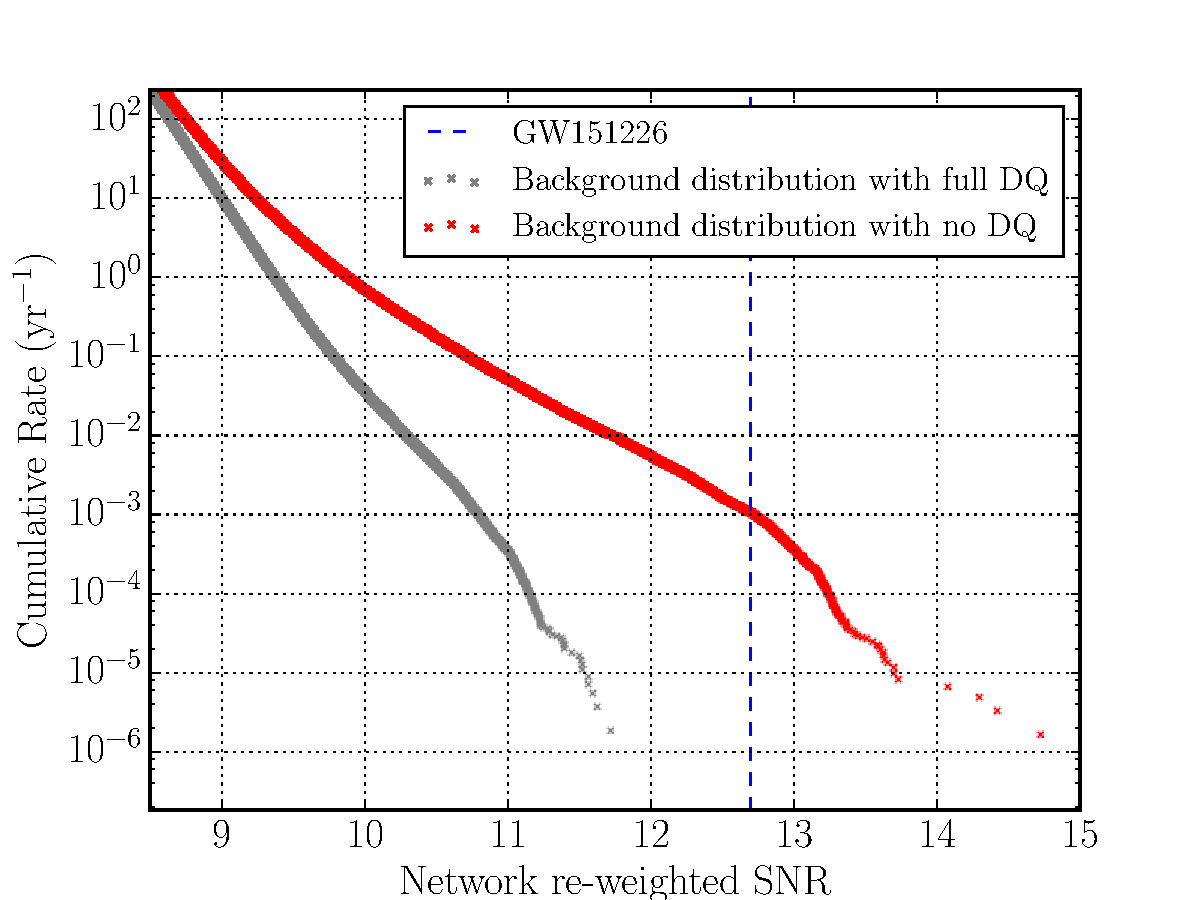
\includegraphics[width=0.495\textwidth]{figures/o1-cbc-dq-paper/bulk_bin_GW151226_DQ_comparison}
  \label{subfig:bulk-bin-gw151226-rate}
  }
  \subfloat[]{
  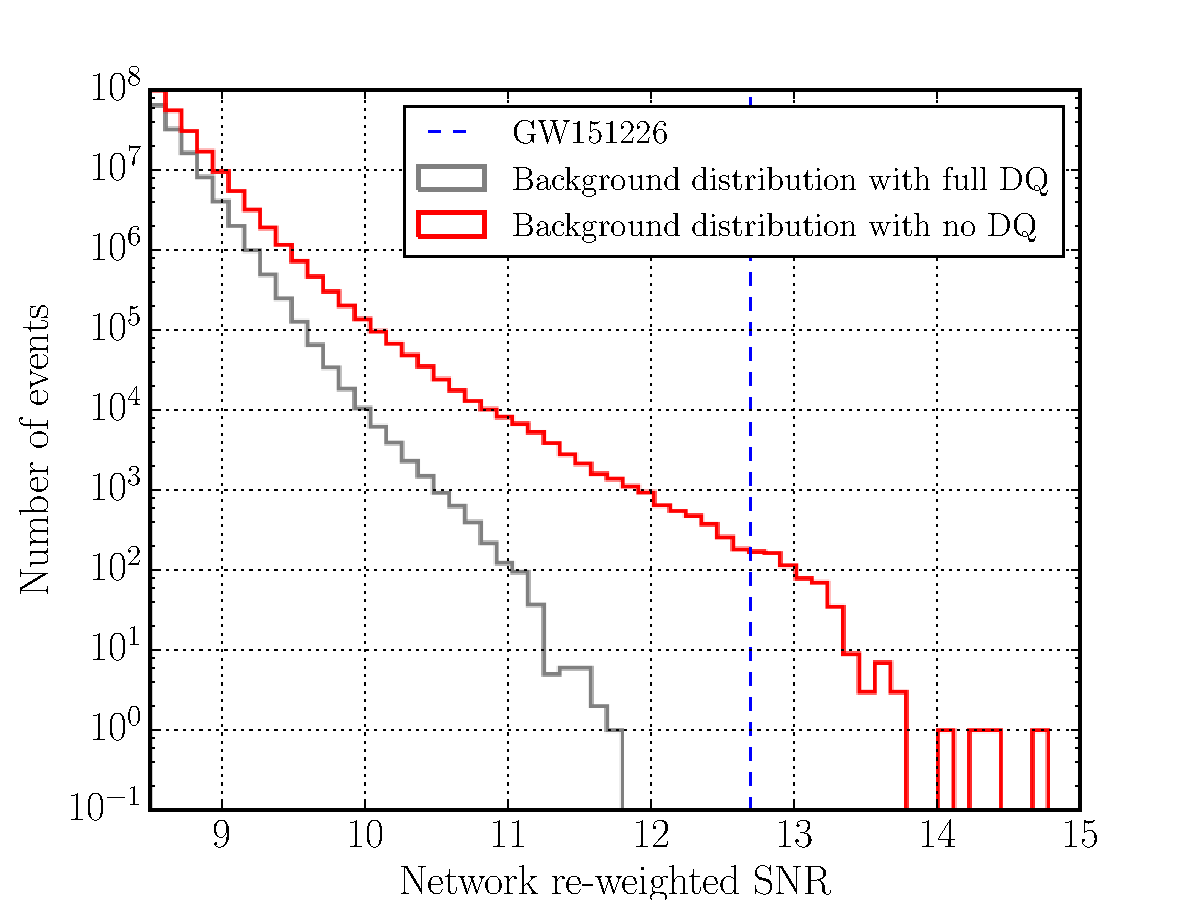
\includegraphics[width=0.495\textwidth]{figures/o1-cbc-dq-paper/bulk_bin_GW151226_DQ_raw_hist}
  \label{subfig:bulk-bin-gw151226-raw}
  }
  \caption[Bulk bin histograms - GW151226 analysis]{The background distribution in the bulk bin before and after applying data quality %
           (DQ) vetoes. % 
           (\ref{subfig:bulk-bin-gw151226-rate}) The cumulative rate of background triggers %
           in the bulk bin as a function of re-weighted SNR. %
           (\ref{subfig:bulk-bin-gw151226-raw}) A histogram of background triggers %
           in the bulk bin. % 
           The red traces indicate the %
           distribution of background triggers without noisy data removed, %
           the gray traces indicate the distribution %
           of background triggers with all data quality vetoes applied. %
           The dotted line indicates GW151226, which was recovered with $\hat{\rho}_{c} =$ 12.7. %
           If no data quality vetoes are applied, the tail of loud background triggers extends to %
           $\hat{\rho}_{c} =$ 14.8 instead of $\hat{\rho}_{c} =$ 11.8. % 
           The impact of this change is apparent when considering GW151226, which is no %
           longer the loudest event in this bin (see Section \ref{sec:GW151226}). %
          }
\label{fig:bulk-bin-far-GW151226}
\end{figure}

\begin{table}[!ht]%
  \begin{center}
    \begin{tabular}{lcc}
      \hline
      Analysis configuration & False alarm rate ($\mathrm{yr}^{-1}$) & False alarm probability \\ \hline
      All vetoes applied & $3.10\times10^{-5}$  & $1.29\times10^{-6}$ \\
      No CAT2 applied & $1.70\times10^{-3}$ & $7.23\times10^{-5}$ \\
      No CAT1 or CAT2 applied & $2.48\times10^{-2}$ & $1.10\times10^{-3}$ \\ \hline
    \end{tabular}
  \end{center}
  \caption[Bulk bin FAR - GW151226 analysis]{Table of bulk bin false alarm rates and probabilities at $\hat{\rho}_{c} =$ 11.3 %
           for several analysis configurations. At $\hat{\rho}_{c} =$ 11.3, the false alarm %
           rate decreases by a factor of 800 when data with excess noise is removed from %
           the analysis. Category 2 vetoes are more effective in this bin, providing a factor % 
           of 54 reduction in false alarm rate.}
  \label{table:GW151226-bulk-far}
\end{table}

\subsection{GW151226}\label{sec:GW151226}

The binary black hole system GW151226 was recovered by the PyCBC pipeline
in the bulk bin with $\hat{\rho}_{c} =$ 12.7 \cite{GW151226}.
The significance of GW151226 was improved by the application of data quality
vetoes. These changes in significance are quantified in Table \ref{table:GW151226-far}.
When all data quality vetoes were applied to the analysis, GW151226 was the loudest
event in the bulk bin and has a false alarm rate of 1 per 183000 years.
If noisy data are not removed from the analysis, GW151226 is no longer the loudest
event in the bulk bin and its false alarm rate increases by a factor of 567
to 1 in 320 years. This
increase takes a clear detection ($>$5$~\sigma$) and reduces its significance to
that of a more marginal detection candidate (3.9$~\sigma$).

\begin{table}[!ht]%
  \begin{center}
    \begin{tabular}{lcc}
      \hline
      Analysis configuration & False alarm rate ($\mathrm{yr}^{-1}$) & False alarm probability \\ \hline
      All vetoes applied & $5.46\times10^{-6}$  & $2.28\times10^{-7}$ \\
      No CAT2 applied & $1.06\times10^{-5}$ & $4.49\times10^{-7}$ \\
      No CAT1 or CAT2 applied & $3.1\times10^{-3}$ & $1.38\times10^{-4}$ \\ \hline
    \end{tabular}
  \end{center}
  \caption[GW151226 FAR]{Table of bulk bin false alarm rates and probabilities of GW151226 for several analysis %
           configurations. The false alarm rate of GW151226 increases by a factor %
           of 567, from 1 in 183000 years to 1 in 320 years, if data with excess noise %
           is not removed from the analysis.}
  \label{table:GW151226-far}
\end{table}

\section{Edge bin}

The background distribution in the edge bin looks dramatically different if data quality
vetoes are not applied. This is not surprising, given that this tuning of the edge bin
is restricted to contain the shortest waveforms with $f_{peak} <$ 100 Hz, which
will have a very short template duration and be susceptible to instrumental transients.
Figure \ref{fig:edge-bin-far-GW151226} shows the background distribution in the edge bin
before and after data quality vetoes have been applied.
The loudest event in this bin with all vetoes applied was at $\hat{\rho}_{c} =$ 15,
which was already inconveniently loud for a search hoping to recover a signal in this
bin. When noisy data are not removed from the analysis, the loudest background event is at
$\hat{\rho}_{c} =$ 18.3, which further restricts the region where a confident
detection could be made.

\begin{figure}[!ht]%
\centering
  \subfloat[]{
  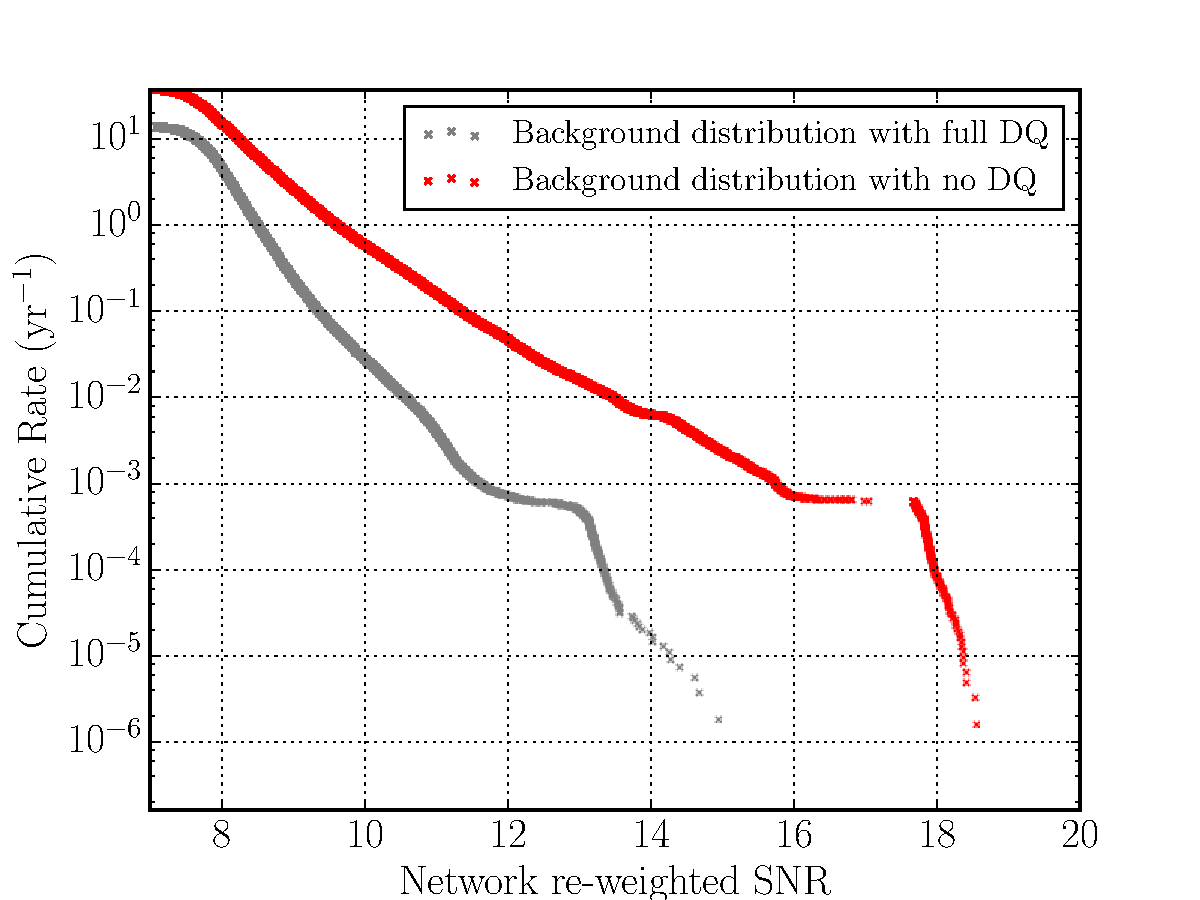
\includegraphics[width=0.495\textwidth]{figures/o1-cbc-dq-paper/edge_bin_GW151226_DQ_comparison}
  \label{subfig:edge-bin-gw151226-rate}
  }
  \subfloat[]{
  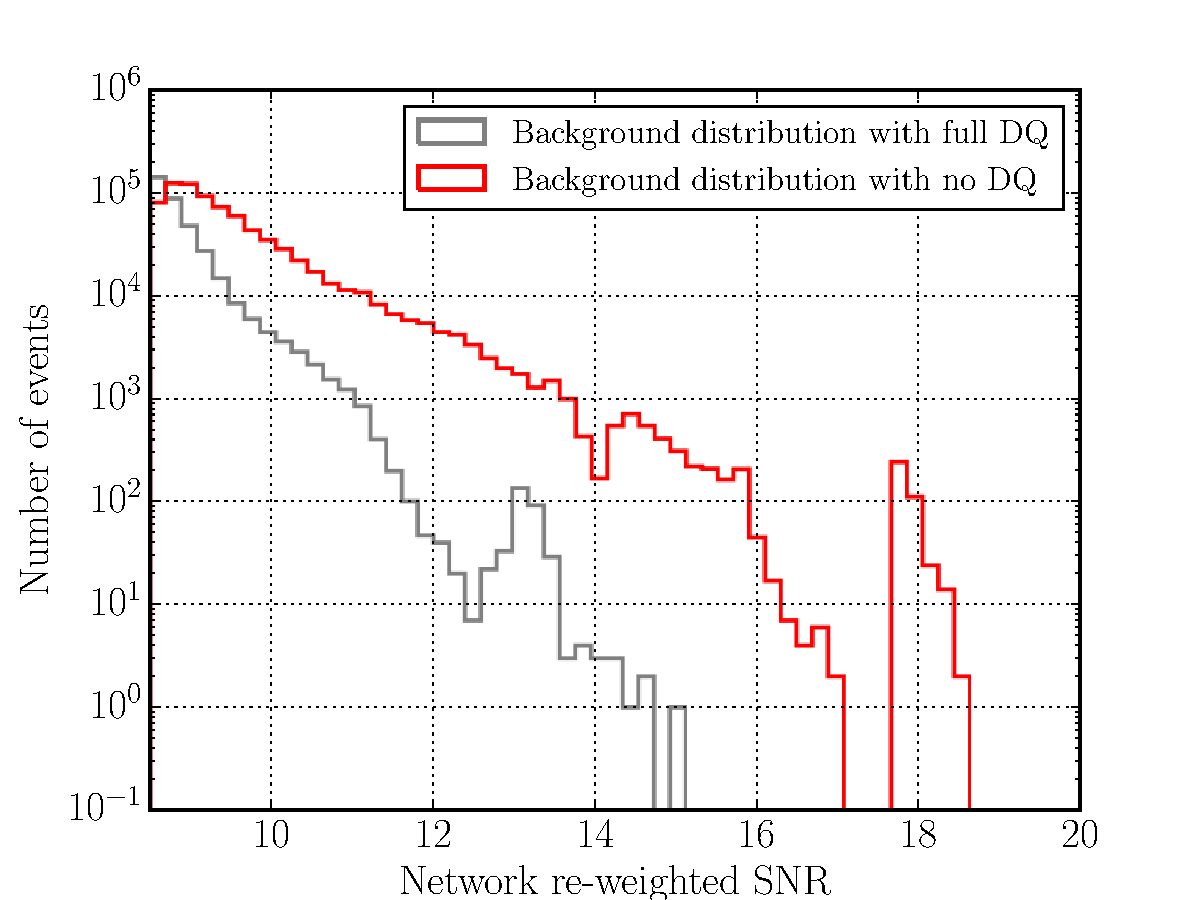
\includegraphics[width=0.495\textwidth]{figures/o1-cbc-dq-paper/edge_bin_GW151226_DQ_raw_hist}
  \label{subfig:edge-bin-gw151226-raw}
  }
  \caption[Edge bin histograms - GW151226 analysis]{The background distribution in the edge bin before and after applying data quality (DQ) vetoes. %
           (\ref{subfig:edge-bin-gw151226-rate}) The cumulative rate of background triggers %
           in the edge bin as a function of re-weighted SNR. %
           (\ref{subfig:edge-bin-gw151226-raw}) A histogram of background triggers %
           in the bulk bin. % 
           The red traces indicate the distribution of background triggers without %
           removing noisy data and the gray traces indicate the distribution %
           of background triggers with all data quality vetoes applied. %
           If noisy data are not removed from the analysis, the tail of loud background  %
           extends to $\hat{\rho}_{c} =$ 18.3.
          }
\label{fig:edge-bin-far-GW151226}
\end{figure}

Further, there is a notable separation between the two background distributions at all
values of $\hat{\rho}_{c}$. This separation can once again be quantified using the
hypothetical detection candidate at $\hat{\rho}_{c} =$ 11.3. Table \ref{table:151226-edge-far}
shows the false alarm rates and probabilities at $\hat{\rho}_{c} =$ 11.3 for various
analysis configurations. When data with excess noise is removed from the analysis, the false
alarm rate at $\hat{\rho}_{c} =$ 11.3 is reduced by a factor of 64.
The application of CAT2 vetoes has an impact in this bin, providing a factor
of 12 reduction in false alarm rate compared to the analysis with only CAT1 vetoes applied.

\begin{table}[!ht]%
  \begin{center}
    \begin{tabular}{lcc}
      \hline
      Analysis configuration & False alarm rate ($\mathrm{yr}^{-1}$) & False alarm probability \\ \hline
      All vetoes applied & $1.70\times10^{-3}$  & $7.08\times10^{-5}$ \\
      No CAT2 applied & $2.16\times10^{-2}$ & $9.16\times10^{-4}$ \\
      No CAT1 or CAT2 applied & $0.108$ & $4.77\times10^{-3}$ \\ \hline
    \end{tabular}
  \end{center}
  \caption[Edge bin FAR - GW151226 analysis]{Table of edge bin false alarm rates and probabilities at $\hat{\rho}_{c} =$ 11.3 %
           for several analysis configurations. The application of CAT2 vetoes %
           has an effect in this bin, providing a factor of 12 reduction in false %
           alarm rate. Applying all data quality vetoes provides a factor of 64 %
           reduction in false alarm rate.}
  \label{table:151226-edge-far}
\end{table}


